\section{Multi-fidelity Data Generation} \label{sec:data_gen}

As with the NASA CRM example in Section \ref{sec:mf_gp_nasa_crm}, three sources of data are used for the Generic T-tail Transport (GTT) test case. 
The lowest fidelity is filled using analyses from the Athena Vortex Lattice (AVL) code, the middle fidelity uses RANS CFD analyses using SU2, and the highest fidelity uses experimental data from wind tunnel campaigns \cite{cunningham_generic_2018,cunningham_preliminary_2018}.
The wind tunnel data was made available through our partnership with The Boeing Company and NASA. 
The lower fidelity data, from AVL and SU2, had to be generated.
This section details the data generation process. 

\subsection{Lowest Fidelity: Vortex Lattice Simulations in AVL} \label{sec:data_gen_avl}
Creating the AVL model required extracting geometry information from Computer-Aided Design (CAD) files for the wind tunnel models. 
Details such as wing, nacelle, and tail locations, airfoil and fuselage cross-sections, and control surface locations were extracted from the provided geometry files. 
These are input into the AVL model to generate the model seen in Figure \ref{fig:gmatt_avl}. 

\begin{figure}
    \center
    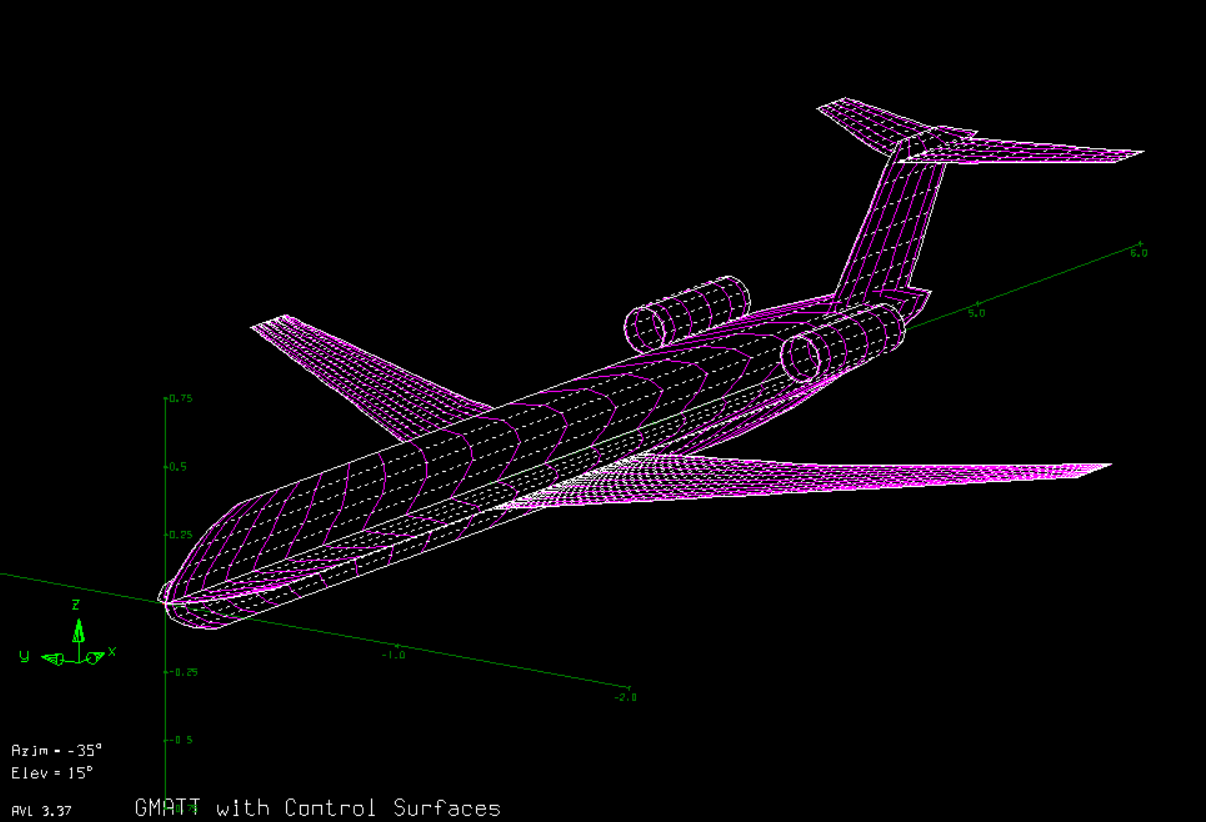
\includegraphics[width=0.65\textwidth]{suthesis/images/gmatt_avl.png}
    \caption{Representation of the GTT design in AVL \label{fig:gmatt_avl}}
\end{figure}

Performing simulations in AVL are relatively inexpensive, taking on the order of a few seconds per analysis. 
This means that large databases can be generated quickly. 
For the baseline aerodynamics, an angle of attack sweep of $-4 ^\circ \leq \alpha \leq 25 ^\circ$ with an evaluation at each angle and an angle of sideslip sweep of $-20 ^\circ \leq \beta \leq 20 ^\circ$ with an evaluation every $4^\circ$, is used. 
This results in 330 required evaluations to define the aerodynamics database.
The same discretization in $\alpha$ and $\beta$ is used for the controls database. 
The control surface deflection sweeps and the total number of AVL evaluations required to generate the controls database are shown in Table \ref{tab:avl_data_points}.

\begin{table}
    \renewcommand{\arraystretch}{1.2}
    \centering
    \begin{tabular}{ c|c|c|c } 
%  \hline
         Control Surface & Deflection Sweep & Number of Deflection Angles & Number of AVL Evaluations \\ 
         \hline
         Ailerons &  $-25^\circ \leq \delta_a \leq 25^\circ$ & 11 & $330 \times 11 = 3630$\\
         Elevator &  $-30^\circ \leq \delta_e \leq 30^\circ$ & 13 & $330 \times 13 = 4290$\\
         Rudder & $0^\circ \leq \delta_r \leq 35^\circ$ & 11 & $330 \times 11 = 3630$\\
         Flaps & $0^\circ \leq \delta_f \leq 45^\circ$ & 10 & $330 \times 10 = 3300$\\
         Spoilers & $0^\circ \leq \delta_s \leq 60^\circ$ & 7 & $330 \times 7 = 2310$\\
         \hline
         & & \textbf{Total Evaluations} & 17160
         
    \end{tabular}
    \caption{List of control surface deflection sweeps and number of AVL evaluations require create the controls database at the lowest fidelity.}
    \label{tab:avl_data_points}
\end{table}

The uncertainty in the AVL analyses is specified using a standard deviation value for each data point. 
AVL uses an extended vortex lattice method to calculate aerodynamic characteristics of lifting surfaces and uses a slender-body model for nacelles and fuselages. 
These simulations solver incompressible potential flow equations which means they ignore compressibility and viscosity effects. 
They cannot model flow separation.
As a result, they are more accurate at lower angles of attack $(\alpha)$, angles of sideslip $(\beta)$, and control surface deflection angles $(\delta_*)$.
To represent these shortcomings in the uncertainty estimates, the standard deviation values are calculated as
\begin{equation}\label{equ:avl_sd}
    \sigma_{AVL}^{C_*(X)} = \max \left \{ 0.1C_*(X=0),~0.002 \left \Vert X \right \Vert \mathrm{range}(C_*) \right \},
\end{equation}
where $C_*$ refers to any coefficient and $X$ refers to the input variables.
Unpacking Equation \ref{equ:avl_sd}, the standard deviation is taken to be the maximum between two terms.
The first term establishes the minimum standard deviation for any coefficient in AVL and is taken to be $10\%$ of the coefficient value at $X =0$. 
Here $X=0$ can mean $\alpha=0, \beta=0$ and/or $\delta_* = 0$, depending on the coefficient.
The second term takes into account the inaccuracy of AVL at higher $\alpha$, $\beta$, and $\delta_*$ by using the $L^2$ norm of the input variables and multiplying it with range of the coefficient.
Using the range allows the equation to generalize to all coefficients, which can be quite different in absolute values.
The $0.002$ factor is a normalizing factor that yields reasonable uncertainty estimates for coefficients.

\subsection{Medium Fidelity: RANS CFD Simulations in SU2}

The medium fidelity level is filled using RANS CFD simulations performed in SU2.
The uncertainty information is provided using the Eigenspace perturbation methodology discussed in Chapter \ref{chap:rans_uq}.
These simulations are computationally expensive so the number of evaluations was limited to a coarse grid-sampling across the $\alpha$ and $\beta$ domain.
Simulations were run for $\alpha \in \left \{ -4^\circ,2^\circ,8^\circ,14^\circ,20^\circ \right \}$ and $\beta \in \left \{ 0^\circ,5^\circ,10^\circ,15^\circ,20^\circ \right \}$.
The results were suitably reflected to create the data for negative sideslip angles. 
Simulation conditions are outlined in \textcolor{red}{Table \ref{}}. 
The SST turbulence model is used for all the simulations.

Modeling stability and control derivatives using CFD is challenging.
For stability derivatives, running unsteady simulations with forced oscillations is required \cite{mcmillin_computational_2019}. 
For controls derivatives, modeling control surface deflections significantly increases the mesh density required to capture surface gaps and the resulting shear layers in the flow. 
Both requirements balloon the computational cost of running simulations to predict these derivatives. 
This precludes the use of CFD data in the controls database and for the stability derivatives.
As a result, the CFD data and associated uncertainties are only used for the baseline force and moment coefficients $\left ( C_L, C_D, C_{SF}, C_l, C_m, \text{and }C_n\right )$

CFD simulations require a mesh with sufficient discretization.
Pointwise is used to generate meshes from the GTT geometry. 
First, a family of three unstructured, half-span meshes are generated.
These meshes are used run a grid convergence study to estimate the numerical discretization error \cite{american_society_of_mechanical_engineers_standard_2009}. 
Details of the meshes are shown in Table \ref{tab:gtt_meshes}.
Some representative images of the mesh are shown in \textcolor{red}{Figure \ref{}}.
The mesh shown is a half-span one.
This is mirrored along the $x-z$ plane to generate a full-span mesh that is used for all simulations involving non-zero $\beta$.
The surface mesh utilizes anisotropic stretching of grid elements along the chord of lifting surfaces. 

\begin{table}
    \renewcommand{\arraystretch}{1.2}
    \centering
    \begin{tabular}{ c|c|c|c|c } 
%  \hline
         Mesh Level & Nodes & Surface Nodes & Wall spacing & Approx y+  \\ 
         \hline
         L3 & $2,281,668$ & $46,621$ & $5\times10^-6 m$ & 1.0 \\
         L2 & $6,722,768$ & $99,644$ & $3.3\times10^-6 m$ & 0.67 \\
         L1 & $19,946,697$ & $209,488$ & $2.3\times10^-6 m$ & 0.23 \\
         
    \end{tabular}
    \caption{Details of the mesh family used to perform numerical discretization error quantification for the GTT configuration.}
    \label{tab:gtt_meshes}
\end{table}

Section \ref{sec:num_vs_turb_error} covered the relationship between numerical discretization error and the turbulence modeling uncertainties. 
The modeling uncertainty was shown to be independent from the numerical discretization error, given a minimum level of mesh refinement that can accurately capture the physics. 
The aim of this grid convergence study is to determine the coarsest mesh that can be used while not introducing significant numerical discretization error. 
\textcolor{red}{Figure \ref{}} shows the results of the grid convergence study and the error bars represent the turbulence modeling uncertainty. 
From the figure we see that while the L3 mesh might be too coarse, between the L2 and L1 meshes the turbulence modeling uncertainty remains consistent. 
This allows the use of the L2 mesh to generate the RANS CFD data, and consequently saves a significant amount of computational resources. 

To estimate the uncertainty injected due to the turbulence model, the eigenspace perturbation methodology introduced in Chapter \ref{chap:rans_uq} is used. 
Accordingly $6$ simulations ($1$ baseline $+~5$ perturbed) are required at each flight condition. 
With $\alpha \in \left \{ -4^\circ,2^\circ,8^\circ,14^\circ,20^\circ \right \}$ and $\beta \in \left \{ 0^\circ,5^\circ,10^\circ,15^\circ,20^\circ \right \}$, a total of $5\times5\times6 = 150$ RANS CFD simulations are run to create the medium-fidelity data and associated uncertainties. 

\subsection{Highest Fidelity: Wind/Water Tunnel Experiments}

The main motivation for using the GTT configuration for this work is the wealth of experimental wind tunnel data that is available \cite{cunningham_generic_2018,cunningham_preliminary_2018}. 
Three experimental campaigns explored different aspects of the aircraft performance characteristics and were performed in the following facilities:
\begin{enumerate}
    \item NASA Langley Research Center 12-Foot Low-Speed Tunnel (12-Foot LST): Focus on stability derivatives and $\alpha$ sweeps,
    \item Boeing North American Aviation Research Tunnel (NAART): Focus on control derivatives and $\alpha$ and $\beta$ sweeps,
    \item Boeing Flow Visualization Water Tunnel (FVWT): Focus on stability derivatives at various values of $\alpha$.
\end{enumerate}
Figure \ref{fig:gtt_exp_images} shows the GTT model in each of the three 
The data from the 12-Foot LST is a subset of the data from NAART and FVWT. 
For this reason, only data from the NAART and FVWT experimental campaigns are used in this work. 

\begin{figure}
    \centering
    \begin{subfigure}[NASA Langley Research Center 12-Foot Low-Speed Tunnel] {
        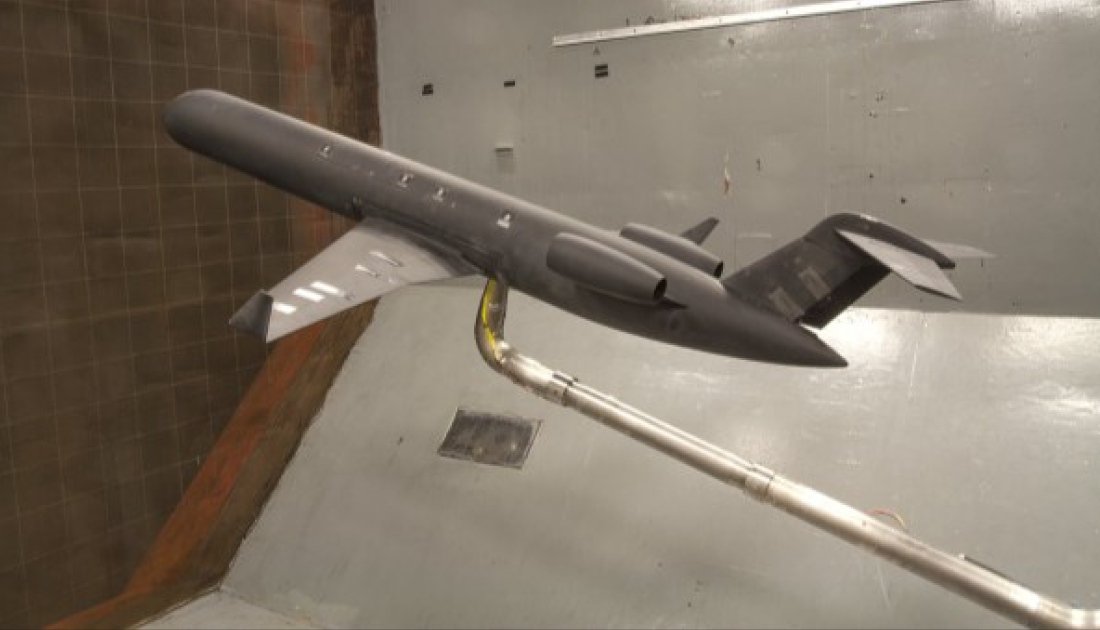
\includegraphics[trim=0 19 0 0, clip, width=.47\textwidth]{suthesis/images/gtt_lst.png} }
    \end{subfigure}
    \hfill
    \begin{subfigure}[Boeing North American Aviation Research Tunnel]{
        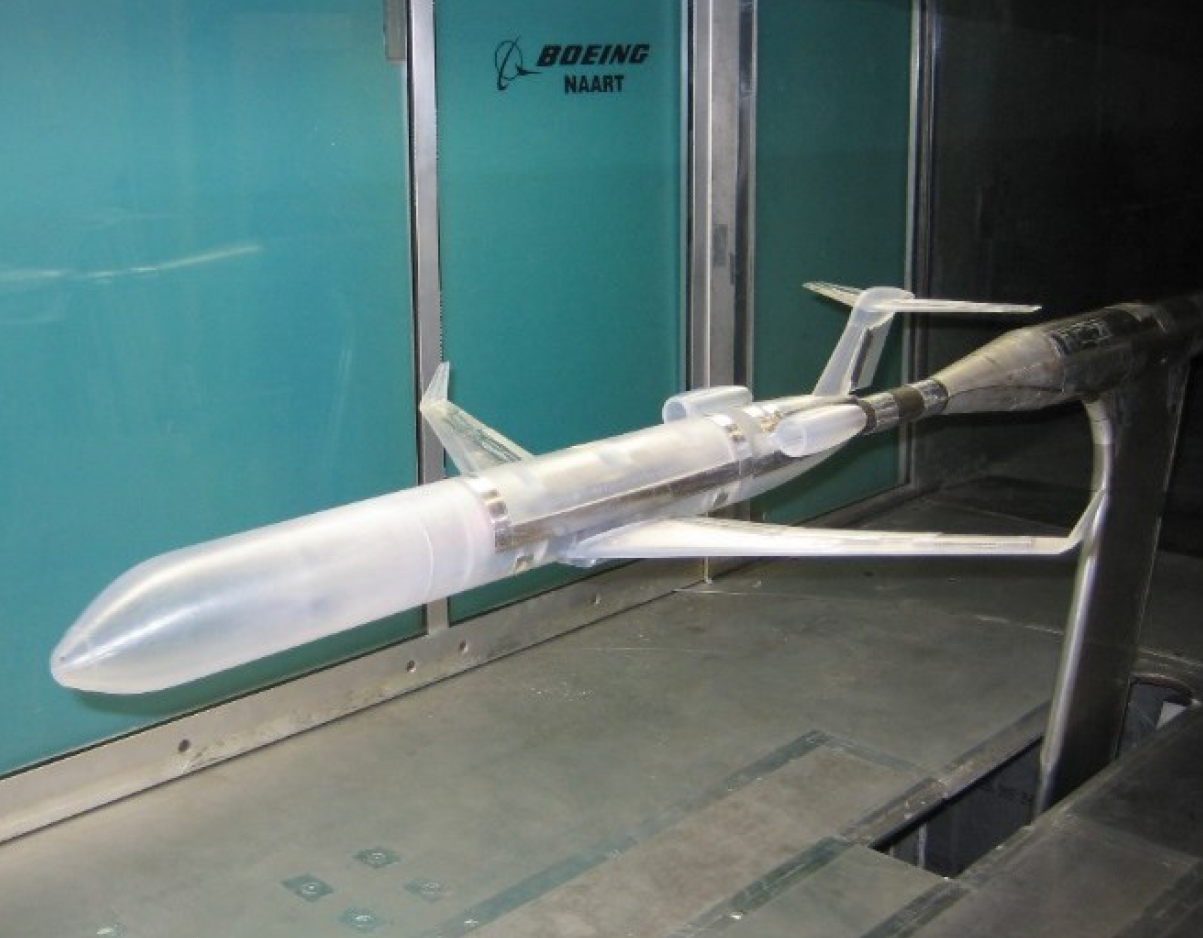
\includegraphics[trim=0 104 0 104, clip, width=.47\textwidth]{suthesis/images/gtt_naart.png} 
    }
    \end{subfigure}
    \hfill
    \begin{subfigure}[Boeing Flow Visualization Water Tunnel]{
        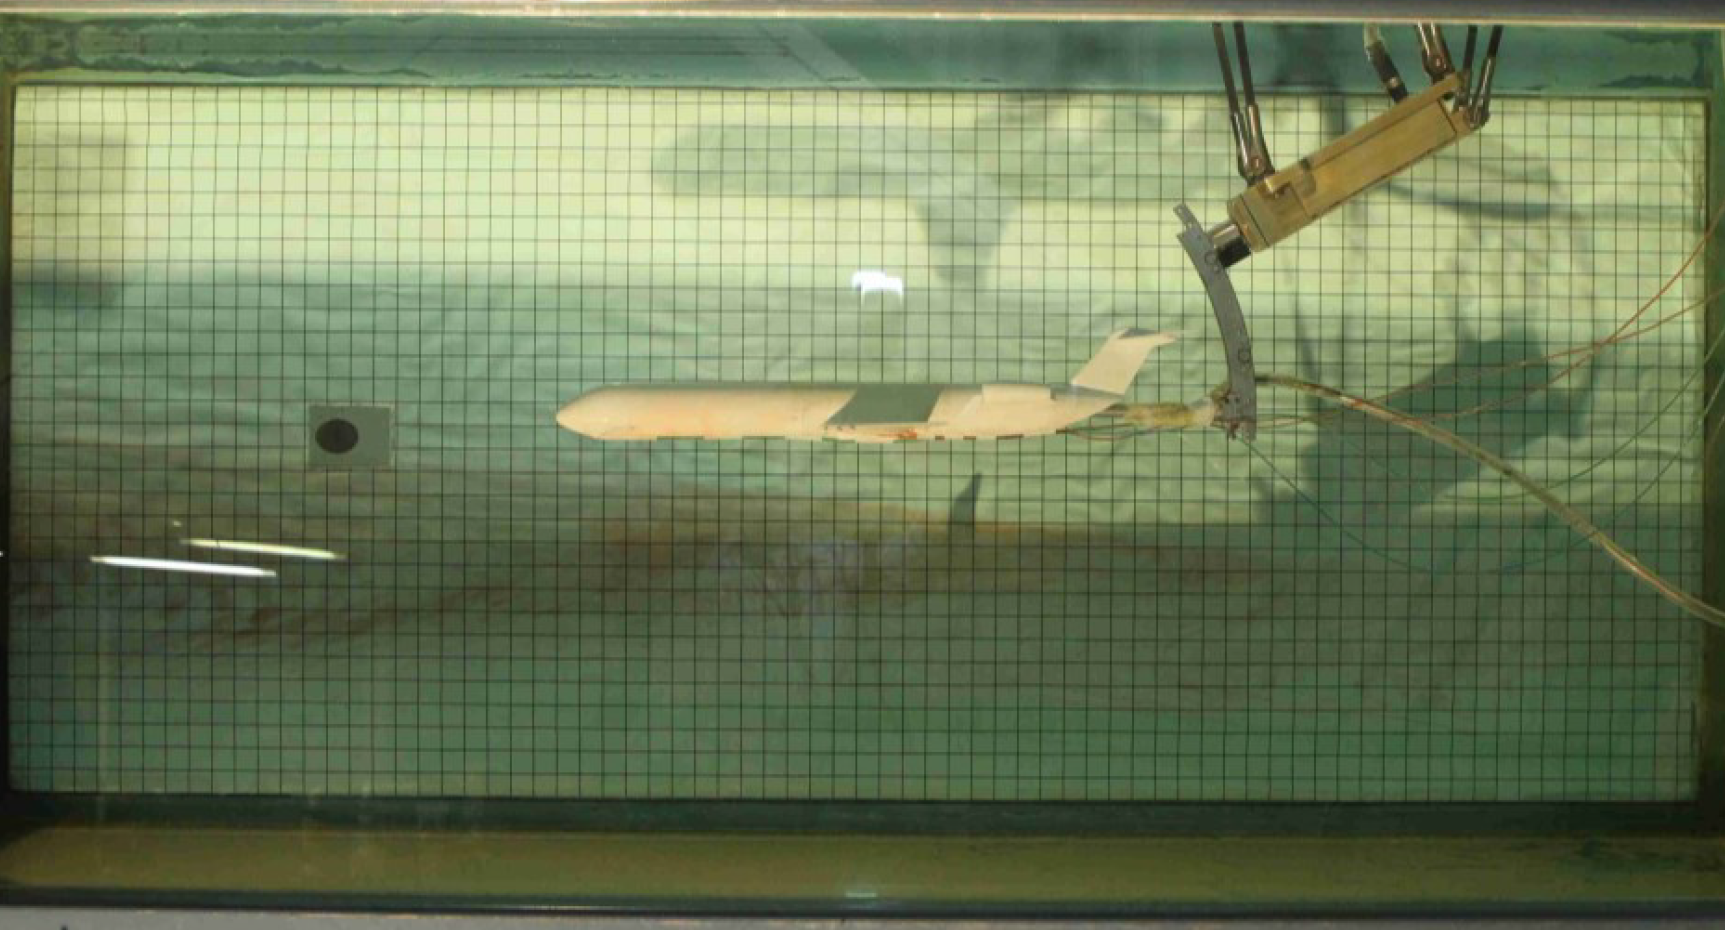
\includegraphics[trim=0 0 0 0, clip, width=.5\textwidth]{suthesis/images/gtt_fvwt.png} 
    }
    \end{subfigure}
    \caption{The GTT model mounted in the various experimental setups that were used.\label{fig:gtt_exp_images}}
\end{figure}

Ideally raw sensor reading from the wind tunnel experiments could be post-processed to determine the uncertainty in the data. 
In its absence, the uncertainty in the aerodynamic coefficients and stability derivatives is estimated as 
\begin{equation}\label{equ:wt_aero_sd}
    \sigma_{WT}^{C_*(X)} = \max \left \{ 1\times 10^{-4},~0.05~\mathrm{range}(C_*) \right \},
\end{equation}
whereas for control derivatives the uncertainty estimate calculation is broken up for each deflection angle
\begin{equation} \label{equ:wt_control_sd}
    \sigma_{WT}^{C_*(\alpha,\beta,\delta=\Delta)} = \max \left \{ 1\times 10^{-4},~0.05~\mathrm{range}(C_*(\alpha,\beta,\delta=\Delta)) \right \}.
\end{equation}

A few guiding principals are employed to reach Equations \ref{equ:wt_aero_sd} and \ref{equ:wt_control_sd}.
The first term in the $\max$ operation forces a minimum uncertainty of $1\times10^{-4}$.
This ensures that the covariance matrices in the Gaussian Process are positive-definite.
In contrast to uncertainties in AVL simulations(Equation \ref{equ:avl_sd}), no great variation in uncertainty is expected due to increased $\alpha, \beta$ or $\delta$ in experimental data. 
Consequently, the uncertainty is not dependent on the magnitude of the input variables, as is the case for uncertainties in AVL simulations. 
Using the range operator allows for a relatively consistent uncertainty estimation across all coefficients, which vary greatly in absolute magnitude. 
For example, pitching moment coefficients are on the order of $10^-1$ while rolling and yawing moment coefficients are on the order of $10^-2$.
The $0.05$ factor means that the expected uncertainty can be estimates as $5\%$ of the range of values for the particular coefficient. 
Control surface deflections cause step changes in the control derivatives as calculated using Equation \ref{equ:control_derivative}.
This necessitates the breakup of the uncertainty estimation according to control surface deflection angle. 
It prevents the higher control derivatives at higher deflection angles from influencing the uncertainty estimates at lower deflection angles.


